\chapter{Literature Review}
\section{Background}
\paragraph{}
Analysis of websites has been carried out in various methods. These forms can be broadly classified into two major categories: qualitative and quantitative methods. Qualitative methods are methods which mainly deal with gaining a deeper understanding about websites and interaction with humans, producing qualitative data. They include content analysis, focus groups, interviews, referrer analysis, user feedback and audience analysis. Quantitative methods employ statistical, mathematical or computational techniques to study websites, producing quantitative data. They include website log analysis, bibliometrics, scientometrics and webometrics.
\paragraph{}
Most web analyses are based on quantitative data. This quantitative data contributes to general knowledge about the usage of a given website. This data can be broken down into numbers and graphs to be interpreted by the website administrators. 
\paragraph{}
Website log analysis is done on logged data e.g. in log files generated from traffic to a website. It is shows details like the number of visits, origin, distribution and their referrals. It is one of the most preferred methods when it comes to website analysis. Most of the current website log analyzers offer a variety of visualization channels to show relevant demographic and geographic data of website visitors. One of the most popular tools to use in this analysis is Google Analytics. This is a tool that allows website administrators to view statistics about their website based on logged data over a period of time. Website administrators use a special code in their web pages and applications to track visitors and generate statistics. Another tool available is AwStats. Unlike Google Analytics, AwStats uses server log files to retrieve statistics about traffic to the website.
\paragraph{}
However, website log analysis is not a very credible measure of website impact. For example, academic websites usually target a small group of people. The number of visits to pages within such a website may not truly reflect the impact on the target group. 
\paragraph{}
Webometrics is another major website analysis method. According to Michael Thelwall, webometrics is “a set of quantitative techniques for tracking and evaluating the impact of web sites and online ideas”. Webometrics encompasses the following fields:
\begin{list}{}{}
\item Informetrics. This is "the study of the quantitative aspects of information in any form, not just records or bibliographies, and in any social group, not just scientists."
\item Bibliometrics. This is "the study of the quantitative aspects of the production, dissemination and use of recorded information"
\item Scientometrics. This is "the study of the quantitative aspects of science as a discipline or
economic activity"
\item Cybermetrics. This is "the study of the quantitative aspects of the construction and use of information resources, structures and technologies on the whole Internet, drawing on bibliometric and informetric approaches"
\end{list}
The terms ‘webometrics’ and ‘cybermetrics’ are often used synonymously though webometrics is a subset of cybermetrics.
\paragraph{}
The main method used in webometrics is link analysis. The reason is that the links to a web site can reveal useful information about how popular it is, which pages or resources are the most popular, why it is popular and where it is popular. Whilst all this information can also be gained from web server log file analysis, the latter can normally only be conducted with permission of a site’s webmaster. In contrast, link analysis can be applied to any web site. This means that link analysis can be used to evaluate a web site by comparing it to its competitors or to similar web sites and can also be used to identify missed audiences for a site. Link analysis has been used extensively to develop algorithms like the Page Rank algorithm, which is used to rank websites in Google’s search engine.
\begin{review_comment}{More info on link analysis}{red}
{More info on link analysis}
\end{review_comment}
\subsubsection{PageRank}
% \begin{review_comment}{pagerank}{orange}
% {
% checkout 10algorithms-08.pdf
% Liu B (2007) Web data mining: exploring hyperlinks, contents and usage Data. Springer, Heidelberg
% Langville AN, Meyer CD (2006) Google’s PageRank and beyond: the science of search engine rankings. Princeton University Press, Princeton
%}
% \end{review_comment}
\paragraph{}
Link analysis on academic institution websites has been inspired by bibliometrics and citation
analysis. A lot of information is published on an academic website. Although some academic papers are published on university web servers, there is a lot of other information in university web sites that is not part of the academic publishing process and is not attempting to directly contribute to the progress of academic knowledge. This will be common knowledge to anyone that has used a university web site, but is nevertheless important. Middleton, McConnell, and Davidson (1999) have proposed, "a model for the structure and content of a university [web] site", claiming that it is in the interests of a university to provide three different types of information.
\begin{list}{}{}
\item Promotional information: advertising services, assets and achievements to potential customers, collaborators and recruits (recruits being both staff and students).
\item Value-added information: providing genuinely useful services to people, encouraging their return and enhancing the institution's reputation as an innovative information provider
\item Utility: to staff and students: information, services and resources that will enable an institution to reach it strategic aims more easily, facilitate external and internal communication and enhance education. This may have the additional benefit of impressing potential customers and recruits, demonstrating the facilities which will be available to them, should they choose to come to the institution.
\end{list}
\paragraph{}
Self-promotion is an important part of the wider process of research, even for individual academics (Hyland, 2003). In other words, departments that do not publicize their work to a more general audience than those that read their published articles are not optimizing their research 'in the round', and may loose out on such things as contacts with industry and new students. The same study also claims that institutions should provide:
...space for scholarly use and learning new ways of exploiting the new medium. Everybody within the institution should have the ability/opportunity to feed into the web site, provided sufficient editorial guidelines are in place.
This promotes a vibrant web culture that encourages usage - seen by many as the raison d'etre of the Internet.
Again, this contribution is unlikely to be surprising for many readers, but it does emphasize that experimentation and variety are natural to university web sites.

\section{Webometrics Ranking of World Universities}
This is one of the most notable implementation of webometrics. It is an undertaking by the Cybermetrics Lab (Spanish National Research Council, CSIC). It analyses and ranks over 20,000 university or academic institution websites. The rankings are published twice a year (January and July) since 2004. The rankings are based on web impact, web presence, openness and excellence.

\subsubsection{Web Impact}
The quality of the contents is evaluated through a "virtual referendum", counting all the external inlinks that the University webdomain receives from third parties. Those links are recognizing the institutional prestige, the academic performance, the value of the information, and the usefulness of the services as introduced in the webpages according to the criteria of millions of web editors from all over the world. The link visibility data is collected from the two most important providers of this information: Majestic SEO and ahrefs . Both use their own crawlers, generating different databases that should be used jointly for filling gaps or correcting mistakes. The indicator is the product of square root of the number of backlinks and the number of domains originating those backlinks, so it is not only important the link popularity but even more the link diversity. The maximum of the normalized results is the impact indicator.

\subsubsection{Web presence}
The total number of webpages hosted in the main webdomain (including all the subdomains and directories) of the university as indexed by the largest commercial search engine (Google ). It counts every webpage, including all the formats recognized individually by Google, both static and dynamic pages and other rich files. It is not possible to have a strong presence without the contribution of everybody in the organization as the top contenders are already able to publish millions of webpages. Having additional domains or alternative central ones for foreign languages or marketing purposes penalizes in this indicator and it is also very confusing for external users.

\subsubsection{Openness}
The global effort to set up institutional research repositories is explicitly recognized in this indicator that takes into account the number of rich files (pdf, doc, docx, ppt) published in dedicated websites according to the academic search engine Google Scholar. Both the total files Both the total records and those with correctly formed file names are considered (for example, the Adobe Acrobat files should end with the suffix .pdf). The objective is to consider recent publications that now are those published between 2008 and 2012 (new period).

\subsubsection{Excellence}
The academic papers published in high impact international journals are playing a very important role in the ranking of Universities. Using simply the total number of papers can be misleading, so we are restricting the indicator to only those excellent publications, i.e. the university scientific output being part of the 10\% most cited papers in their respective scientific fields. Although this is a measure of high quality output of research institutions, the data provider Scimago group supplied non-zero values for more than 5200 universities (period 2003-2010). In future editions it is intended to match the counting periods between Scholar and Scimago sources.

\section{Indicators}
These four indicators give an academic institution’s visibility and activity. The visibility is gotten from impact and accounts for 50\%. The activity is comprised of web presence, openness and excellence and accounts for 50\%. The Webometrics ranking methodology comprises of four different parameters; Visibility (50\% (link visibility 20\% and G-factor 30\% as of July 2011)), Size (20\%), Rich Files (15\%), and Scholar (5\%) and Scimago (10\%).
\begin {review_comment}{pie chart img}{orange}
{get better pie chart}
\end{review_comment}
\begin{figure}
	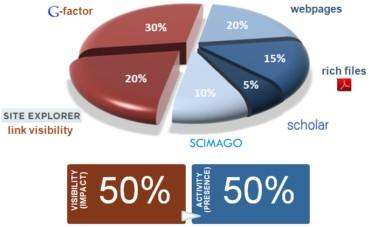
\includegraphics[width=\linewidth,scale=0.5]{../static/img/analysis_model.jpg}
	\caption{Webometrics university ranking methodology. Source :}
\end{figure}
\subsubsection{Visibility}
The total number of unique external links received (inlinks) by a site can be only confidently obtained from Yahoo Search. Results are log-normalised to 1 for the highest value and
then combined to generate the rank.
\subsubsection{Size}
Number of pages recovered from four engines: Google, Yahoo, Live Search and Exalead. For each engine, results are log-normalised to 1 for the highest value. Then for each domain, maximum
and minimum results are excluded and every institution is assigned a rank according to the combined sum.
\subsubsection{Rich Files}
After evaluation of their relevance to academic and publication activities and considering the volume of the different file formats, the following were selected: Adobe Acrobat (.pdf), Adobe PostScript (.ps), Microsoft Word (.doc) and Microsoft Powerpoint (.ppt). These data were extracted using Google and merging the results for each filetype after log-normalising in the same way as described before.
\subsubsection{Data storage}
Data collected from the websites crawled had to be stored for future analysis. Storage was possible in two ways : 
\begin{enumerate}
\item \itemhead{Traditional relational databases}
They provide the most common solution for storing data. They aim to provide data integrity even though this is done while compromising performance. The web crawler collects numerous pages per second on a good network connection. Therefore, the crawler generates alot of data in a short amount of time. This would lead to the system hitting the database with inserts multiple times per unit time and the RDBMS trying to validate and ensure data integrity. This would undoubtedly develop into a bottleneck for the system in terms of scalability and speed.

\item \itemhead{Flat files}
They provide the simplest solution of the three choices. The format chosen to store the data was JSON. The data was stored as JSON lines not JSON objects. This was done to ensure the reading and writing of the files was done on a line by line basis not as one object to ensure minimal memory consumption and I/O access delays. The system at first used json files to store the data though it became evident that file location would become a thorny issue. 

\item \itemhead{NoSQL databases}
They come in different forms e.g. document-oriented databases, graph databases e.t.c. They were developed as a solution to the constrictions of traditional SQL databases'.

\end{enumerate}
\begin{review_comment}{comparisons}{red}
{
    comparison between sql and nosql databases
    reasons for using flatfiles (json)
    comparison between document and graph databases
}
\end{review_comment}
